\section{system design}

\begin{figure}[htb]
  \centering
    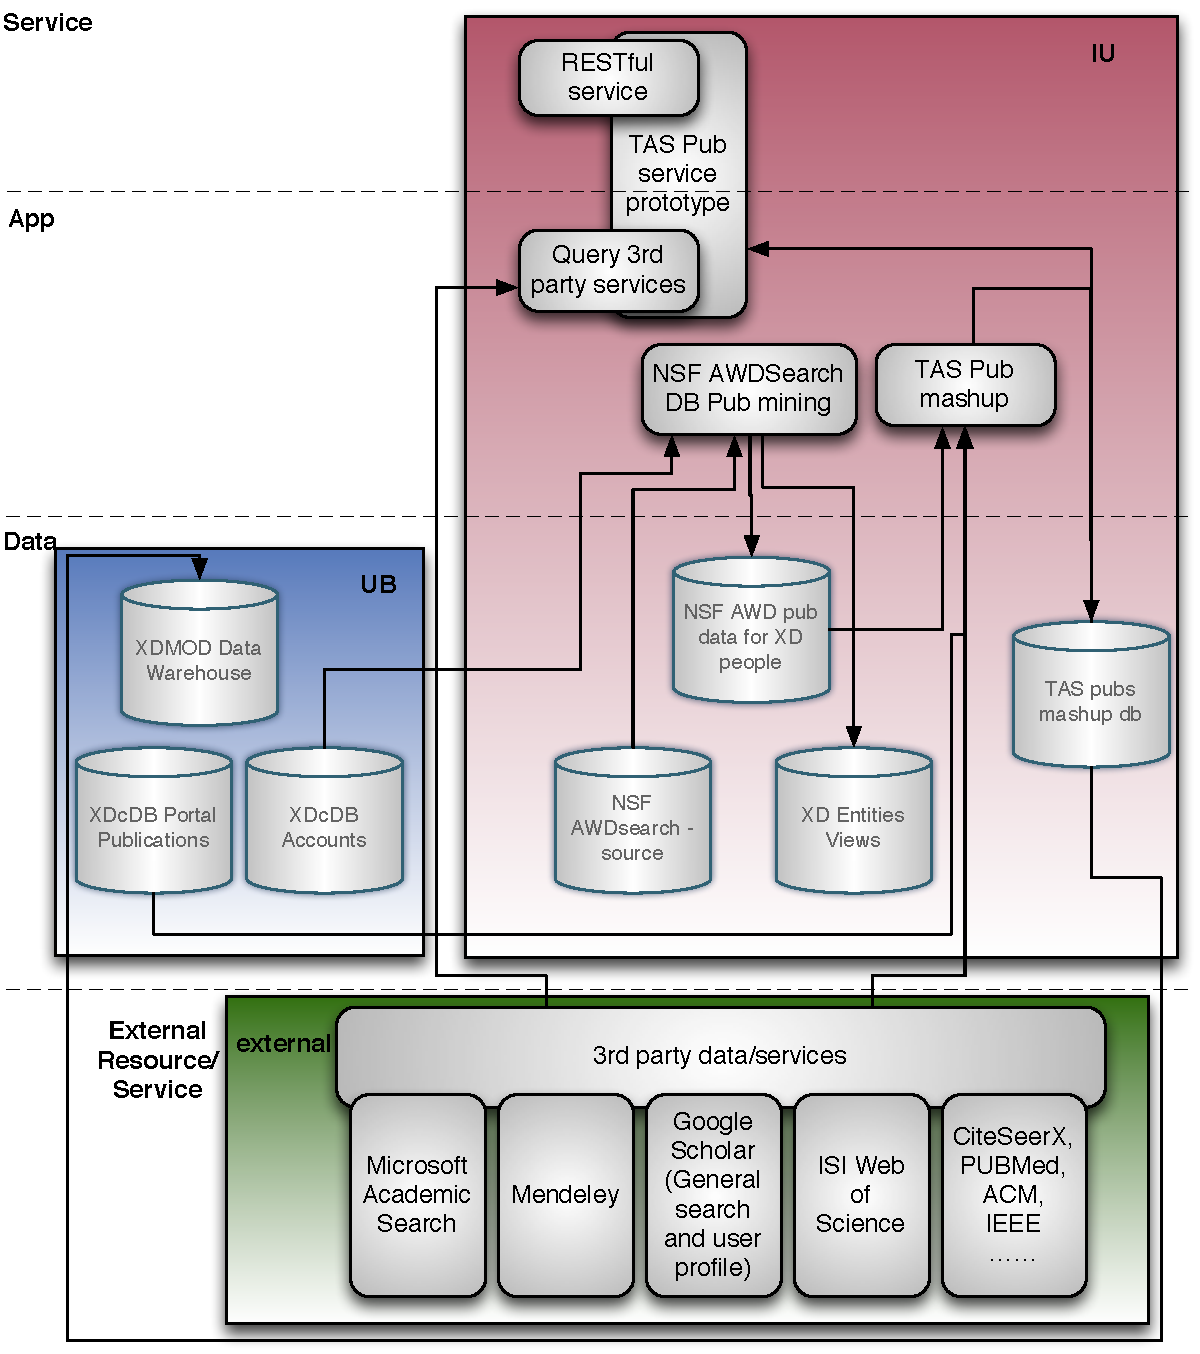
\includegraphics[width=1.0\columnwidth]{images/tas-arch.pdf}
  \caption{The Architecture of the Framework}\label{F:tas-arch}
\end{figure}
 
We have designed a software framework to support the impact measuring. It is a largely distributed (involves IU, UB, NCSA and other external resources e.g.) service-oriented system  that consists of publication and citation data retrieval (e.g., from Google Scholar and ISI Web of Science), parsing and processing while correlating data from various databases and services (e.g., XSEDE central database and POPS database); the metrics generation and analysis system for the different aggregated levels (users, projects, organization, Field of Science (FOS) ); as well as a presentation layer using a light weight portal in addition to exposing some data via RESTful API.

Fig \ref{F:tas-arch} shows the layered system architecture, with an emphasis on relationships between related components especially among the databases. In general we obtain the publication data for each XSEDE user, and then retrieve the citation data for each publication. The data are originally collected per user and per publication basis, but would be aggregated based on organization, XSEDE project/account, Field of Science (FOS), etc. for the metrics generation and analysis. When correlating the data to the input, in this context the Service Units (SUs) awarded by XSEDE, the analysis could reveal patterns and trends of how XSEDE can impact the sciences and potentially helps to achieve better return of investment.

While we are using the system to analyze the scientific impact of XSEDE, the framework itself is flexible enough that could be easily adapted to other similar systems for impact measure and analyses.
